\chapter{Experiment and Web application}
%This thesis will try to determine questions regarding micro-tasks involving geospatial data. 
%There is little research on how inexperienced individuals solve micro-tasks when the tasks involve map interaction. To the authors best knowledge, little, if any, research has been conducted on micro-tasks involving geospatial interpretation and analysis. 
This chapter will introduce the developed experiment and the implemented web-application hosting the experiment. The web application containing the experiment generates the data for the analyses. A pilot-test of the web application is used to secure the usability and discover weaknesses in the implementation. How the pilot-test was executed and some preliminary results, is also presented in this chapter. At last, there is a section about how to determine the sample size.  
%The gathered data from the experiment will be used to get more knowledge about micro-tasks involving geospatial tasks, both how to best partition the large geospatial task and how well individuals solves the tasks based on their background. 
%The experiment will be administered through a Self-Administered Questionnaire, where the questions will be located in a web-application developed and implemented by the author. When doing questionnaire designed survey, a key factor is to keep the questions short, simple, and clearly worded [\citep{Kitchin2000}, p. 52].

%This thesis will try to answer questions regarding micro-tasks containing geospatial data. Is it safe to assume that individuals, both experienced and inexperienced, can interpret and analyze geospatial data presented to them on both map and in tables correctly? Can individuals with little experience in working with geospatial data and map solve geospatial micro-tasks? To the authors best knowledge, little, if any, research has been done on micro-tasks involving map interaction and geospatial interpretation and analysis. 
%Our first sample application asks users to identify which object does not belong in a collection of items. This kind of task requires both image- and semantic-classification capability %http://dbarowy.github.io/AutoMan/

\section{Experiment}\label{sec:experiment}
% In general, questionnaires are used to generate quantitative data, which is later used to calculate statistical information [\citep{Kitchin2000}, p. 48]. The experiment is used to generate data and to answer the research hypothesis. 
In the experiment, the participants answer two questions, representing two micro-tasks, on three different tasks. The first question asks the participant to click on the footprint layer that fits the shape of the building shown on the base map best. In the second question, it asks the participant to click on the row that gives the most informative information about an arbitrary building. The three tasks in the experiment will ask the same two questions, but each task varies the number of elements the participant has to answer before the micro-task (question) is complete. This section will introduce the two micro-tasks and the three tasks. It will also describe how the building footprints, used in question one, was developed. 

\subsection{The two micro-tasks}\label{sec:experimentquestions}
%\cite{Gadiraju2015} categorize the top-level crowdsourced tasks, after analyzing platforms as MTurk and CrowdFlower. It resulted in three relevant classes within geospatial data: \textit{1)Verification and validation}, \textit{2)Interpretation and analysis} and \textit{3)Content creation}. There are examples of all three task classes in geospatial crowdsourcing. 
%During imports of large datasets into OpenStreetMap, crowdsourcing is used to validate the new data (\ref{sec:buildingimport}). 
%In humanitarian OpenStreetMap, they map areas during a crisis to support the help organizations through crowdsourcing, creating valuable content to the workers in the field (\ref{sec:taskingmanager}). In a machine learning process, they are starting to use micro-tasks to both validate the created data and also create data sets to train the algorithms (\ref{sec:whyneedhumans}). \textit{Interpretation and analysis} tasks rely on the individual to use their interpretation skills during task completion. 
%The micro-tasks given in the building imports from section \ref{sec:buildingimport} was primarily interpretation and analysis tasks \citep{Erichsen2016}. When developing the three  The experiment conducted in this thesis use \cite{Gadiraju2015} three classes and the building imports described in \cite{Erichsen2016} as guidance when the two micro-tasks given to the participants was developed.  

The first question (micro-task) asks the participant to click on the color that fits the shape of the marked building(s) on the map best. Here the participant is given two footprint layers covering a building. The participant needs to determine which of the footprints that fit the shape of the building shown on the base map best. This task is highly relevant during building imports and data validation if one has two overlapping geometry layers. This question is inspired by the micro-tasks given in the building imports from section \ref{sec:buildingimport}. The import process can not be done fully-automatic in OpenStreetMap, and a human task can be to validate which footprint fits the building shape best. Question one displayed on the web application is presented in figure \ref{fig:q12}. In this example, the participants have three buildings to select before the micro-task is completed. 

\begin{figure}[H]
	\centering
	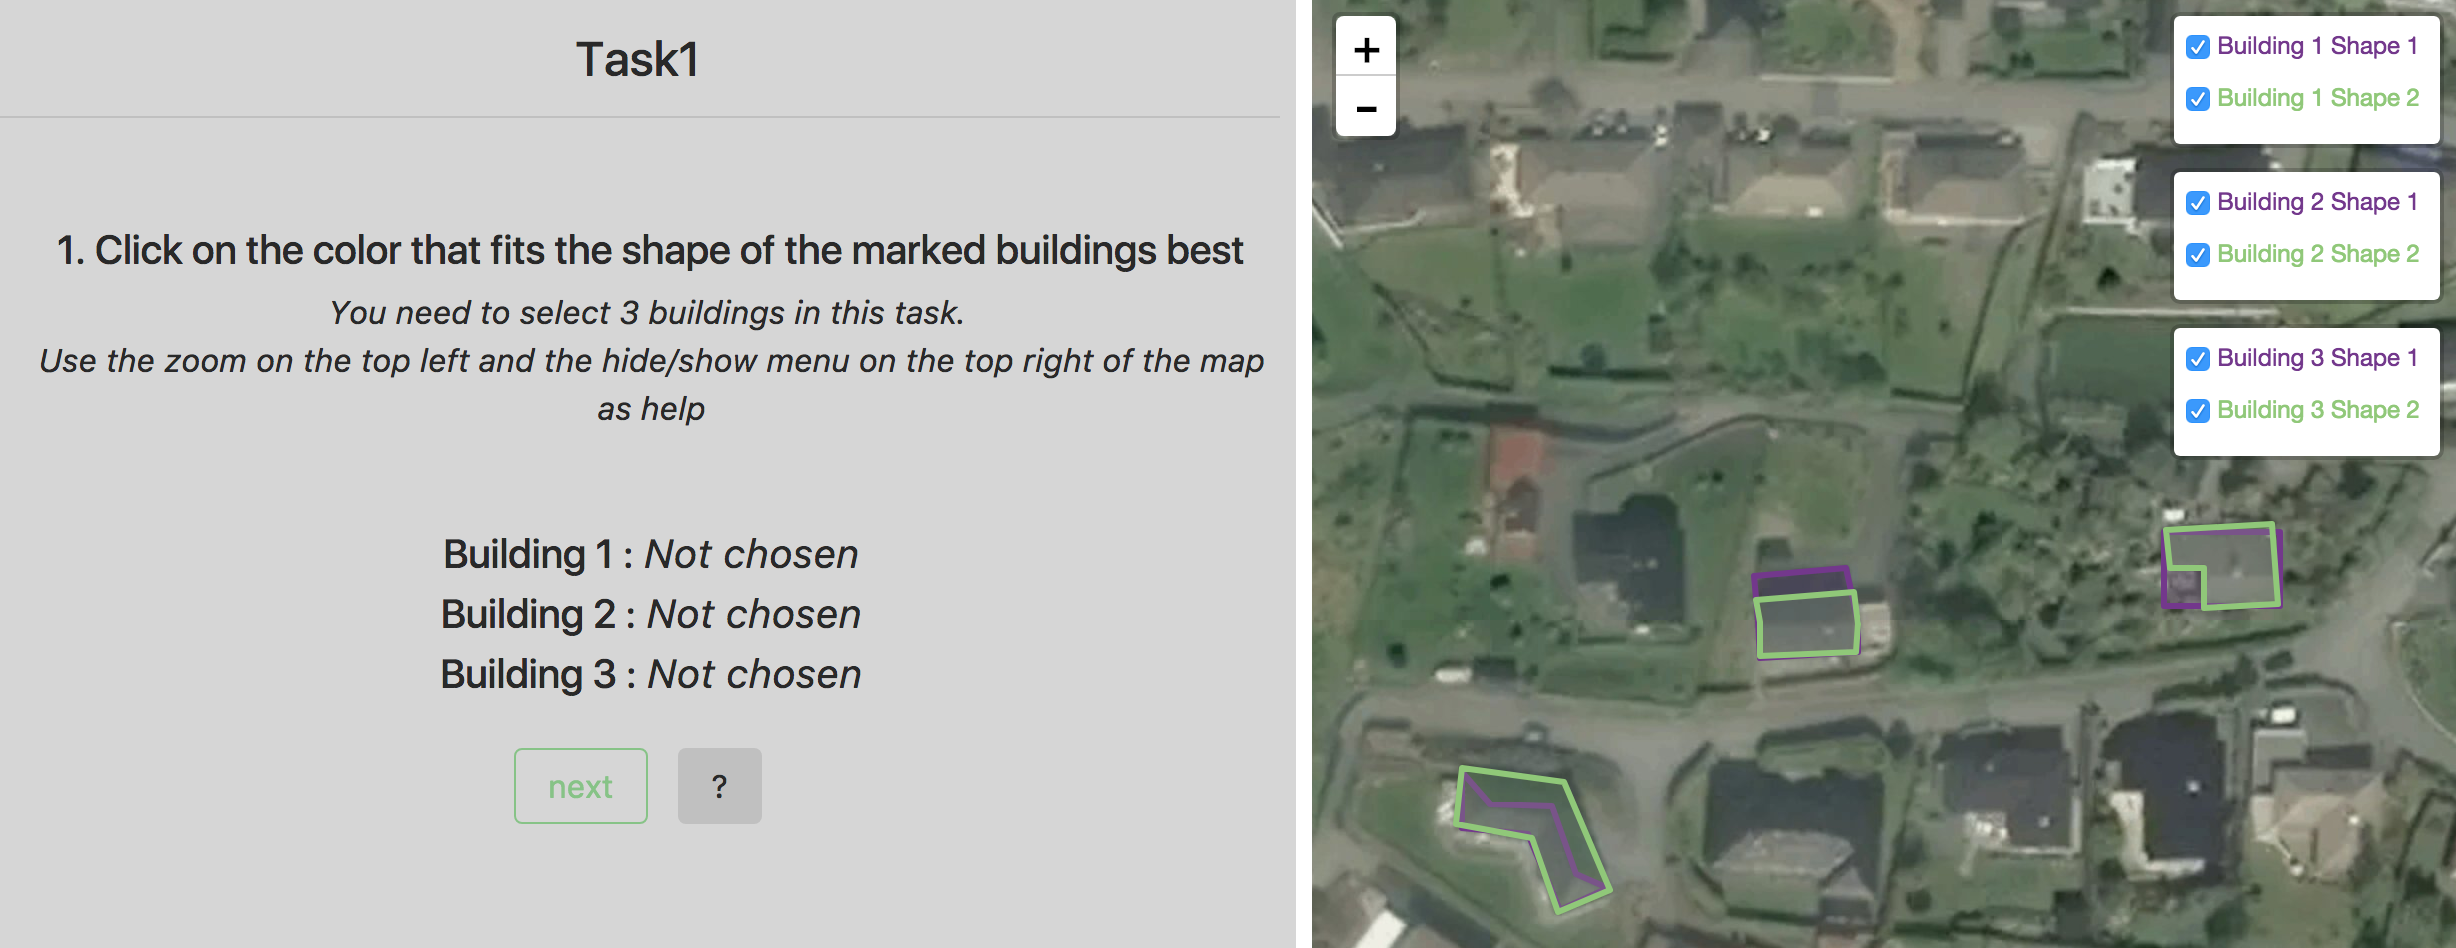
\includegraphics[width=0.8\linewidth]{fig/q1_2}
	\caption{Question one as it is displayed in the web application during task B}
	\label{fig:q12}
\end{figure}

The second question (micro-task) asks the participant to select the most informative row(s) that describe random buildings best. Question two is an interpretation task where the participant needs to interpret the information written in the table to decide which row(s) gives the most informative information about an arbitrary building. This is task is not easy to solve automatic through a script. The correct answer will vary between buildings and what information is present. In figure \ref{fig:q22} question two is displayed in the web application. In this example, the participant has to select three rows from the table before the micro-task is completed. 

\begin{figure}[H]
	\centering
	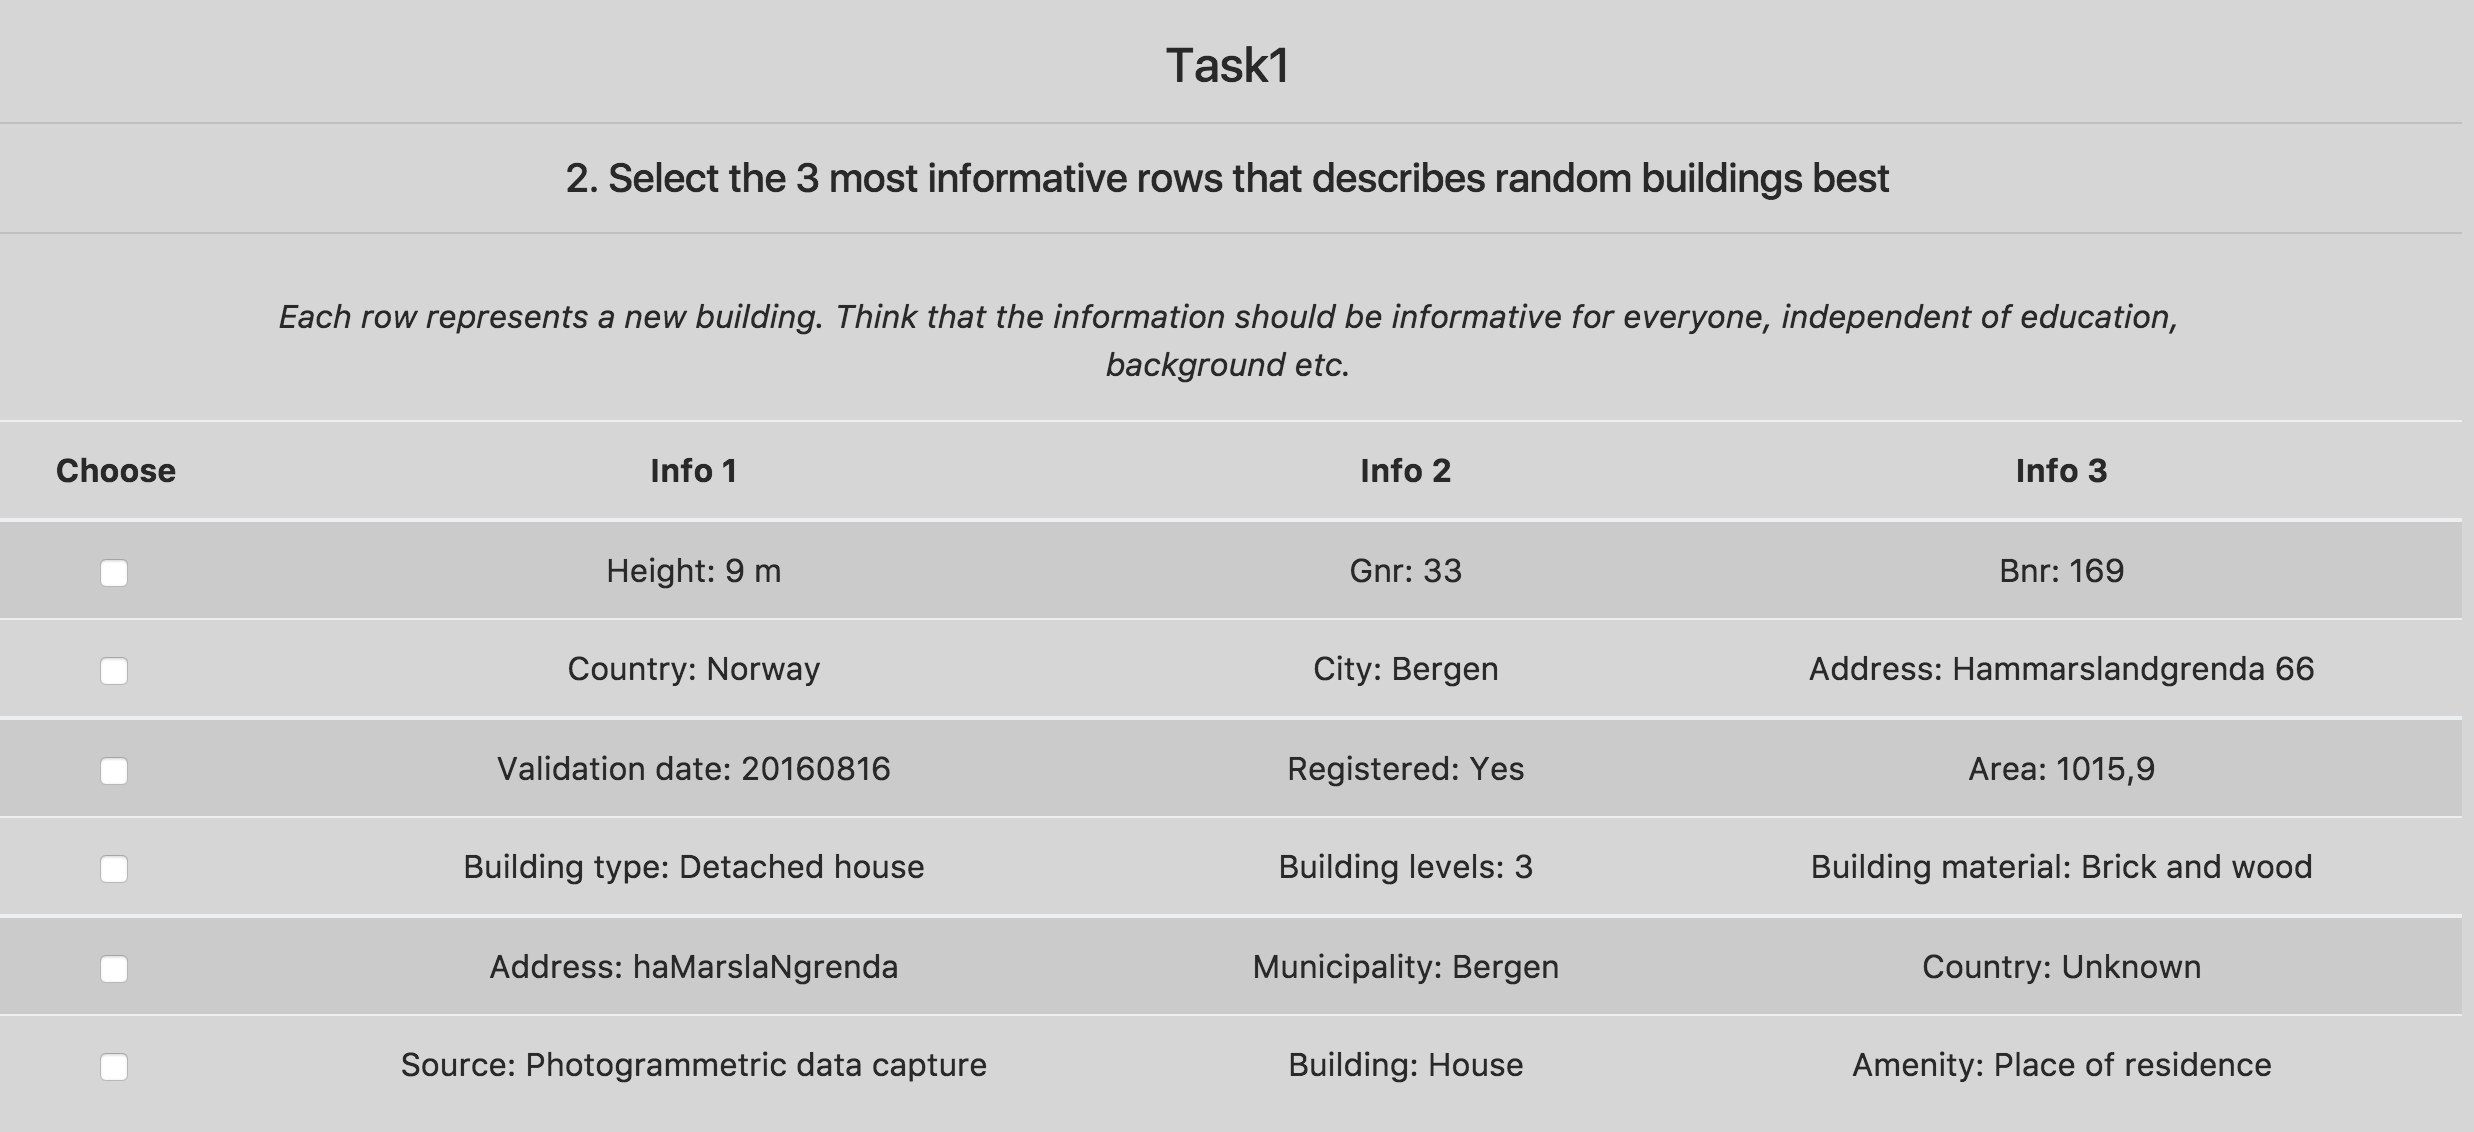
\includegraphics[width=0.8\linewidth]{fig/q2_2}
	\caption{Question two as it is displayed in the web application during task B}
	\label{fig:q22}
\end{figure}

\subsection{The three experiment tasks}\label{sec:experimenttasks}
The experiment consists of three different tasks, in addition to a training task. It will explore how the amount of workload demanded in each task influence the task performance. In this thesis, the number of task elements in each micro-task will determine the amount of workload. The task complexity and workload is dependent on mental effort and cognitive load, as mentioned in section \ref{sec:taskcomplexity}. Each task contains six elements, but the tasks vary how many elements that are necessary to answer before the micro-task is completed. One task will serve the participant with micro-tasks containing one element, called task A. This task demands the smallest cognitive load and the lowest complexity. The next task will serve the participant with micro-tasks containing three elements, called task B. This number is just below the limit of how much information humans can process \citep{Mandler2013}. The last task will serve the participant with micro-tasks containing all six elements, called task C. This number exceeds the human capacity when processing information according to \cite{Leppink2014a}. An illustration of the tasks is shown in figure \ref{fig:illustrationmicrotasks}.

\begin{figure}[H]
	\centering
	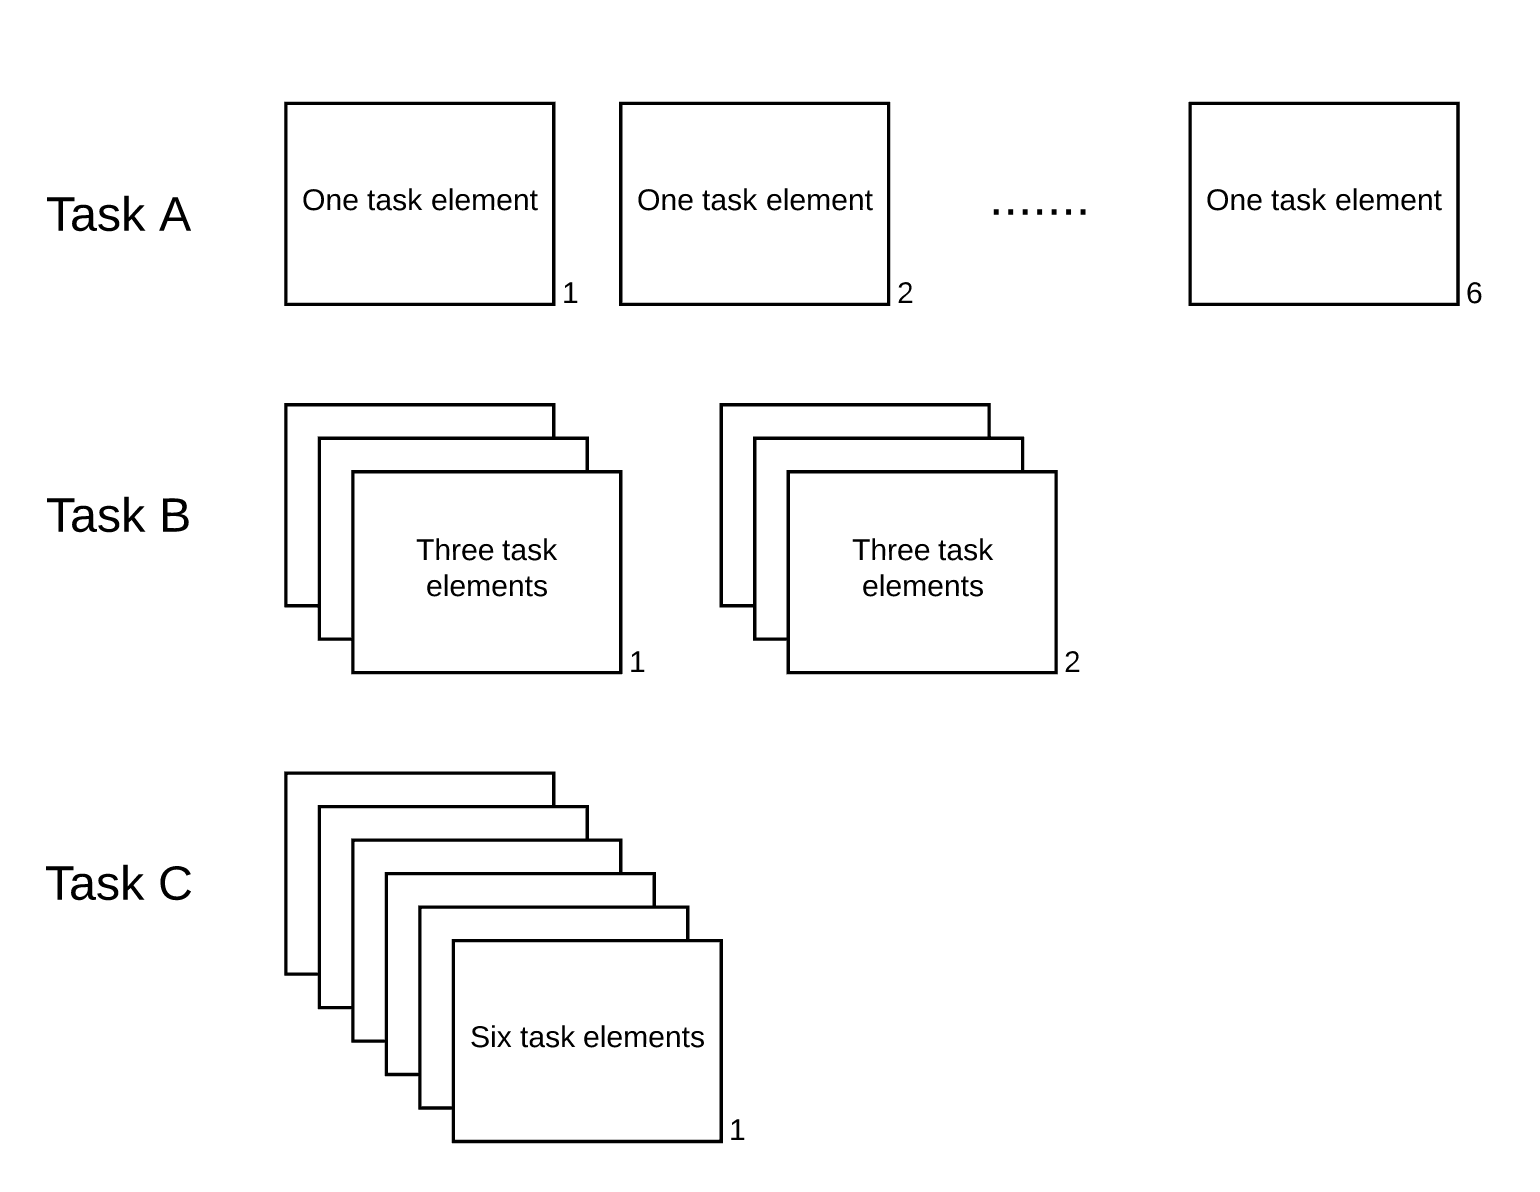
\includegraphics[width=0.7\linewidth]{fig/illustration_microtasks}
	\caption{Illustration of the three tasks given in the experiment}
	\label{fig:illustrationmicrotasks}
\end{figure}

By choosing three elements in one task and six elements in the other task, this paper can determine if the theories about the limited capacity of the human brain also apply to micro-tasks involving geospatial data. One task will only contain one element as a minimum cognitive load task. The three tasks can help answer how many elements a human can process at the same time without impacting the quality of the result. The goal is to determine a preferred number of elements to include in a micro-task. This information can be useful when developing micro-tasks to achieve adequate task progress as well as accurate results.

The “magical” number of four has been demonstrated to limit much of human information processing \citep{Mandler2013}. It is said that polygon comparison demand medium cognitive load \citep{Kiefer2016}, which is what the participants do in the first question in the experiment. \cite{Kiefer2016} argues that high cognitive load may lead to less efficient map reading and spatial orientation, as well as decreased spatial learning. Since polygon comparison demand medium cognitive load, question one should at least not be too demanding on the one- and the three elements micro-tasks. 

A worry is that inexperienced participants will have a larger struggle than the experienced participants.  By dividing the participants into experienced and inexperienced categories, the results from the experiment can help determine if geospatial micro-tasks are too demanding for the inexperienced individuals. 

\subsection[Building shapes]{Determining the building footprints used in question one}

%Remote sensing is a tool or technique for extracting information about objects or geographic areas. All remote sensing images are subject to some form of geometric distortions. The distortions depend on how the data are obtained \citep{Toutin2004}.  In Norway, most remote sensing images are analysed manually. This is also the case in OpenStreetMap. When using remotely sensed images to create for instance building footprints, it's important to be aware of the distortions in these images. 

According to \cite{Fan2014}, there was over 77 million buildings in the OpenStreetMap (OSM) database in 2013. A study of the geometries of building footprints in the city Munich reveal a huge diversity in the geometries \citep{Fan2014}, and this is probably not the only city with this kind of diversity. The \cite{Fan2014} paper used four criterion: \textit{completeness}, \textit{semantic accuracy}, \textit{position accuracy} and \textit{shape accuracy}, to evaluate the quality of the building footprints in OSM. In the creation of the two footprints representing the buildings used in question one, the quality criterion shape- and position accuracy was emphasized. The goal is to create shapes that match realistic cases that occur for instance in OSM. 

Shape accuracy evaluates how well the layer matches the building in an aerial image. \cite{Fan2014} mentions two main reasons to why building footprints are simplified in OSM. The first reason is the difficulties following building details when looking from a bird's eye view. The second reason is the limited resolution of the Bing aerial image used in OSM during digitalization. In question one, two footprints is drawn with one of them matching the building shape better than the other. The participant has to use an base map to determine which layer fits the building best. This will test if the participants manage to make correct shape judgments by only using an base map as a reference. 

\begin{figure}[H]
	\centering
	\begin{subfigure}[b]{0.32\textwidth}
		\centering
		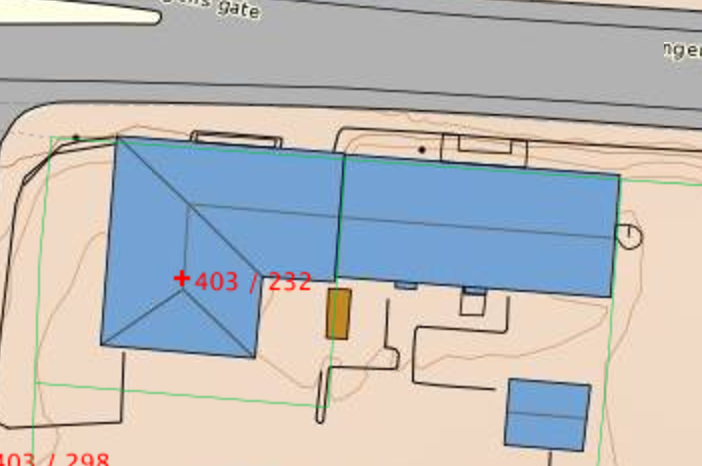
\includegraphics[width=\linewidth]{fig/build1}
		\caption{Official building footprint}
		\label{fig:build1}
	\end{subfigure}
	\begin{subfigure}[b]{0.32\textwidth}
		\centering
		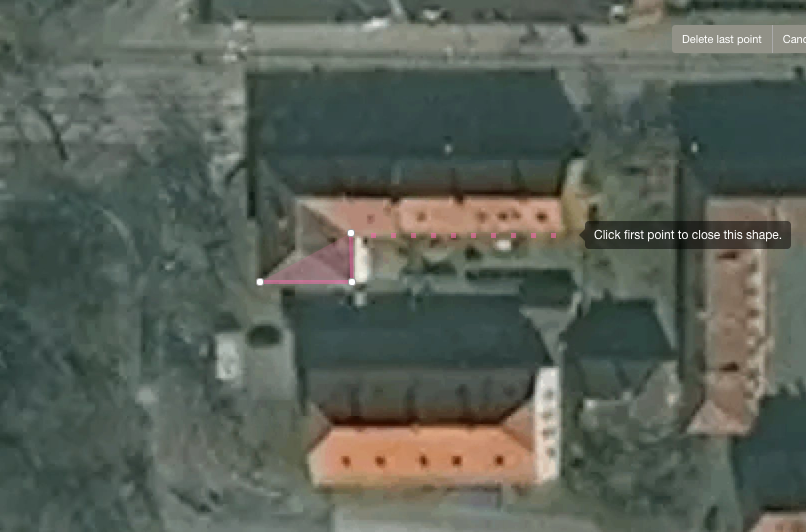
\includegraphics[width=\linewidth]{fig/build2}
		\caption{Drawing a footprint}
		\label{fig:build2}
	\end{subfigure}
	\begin{subfigure}[b]{0.32\textwidth}
		\centering
		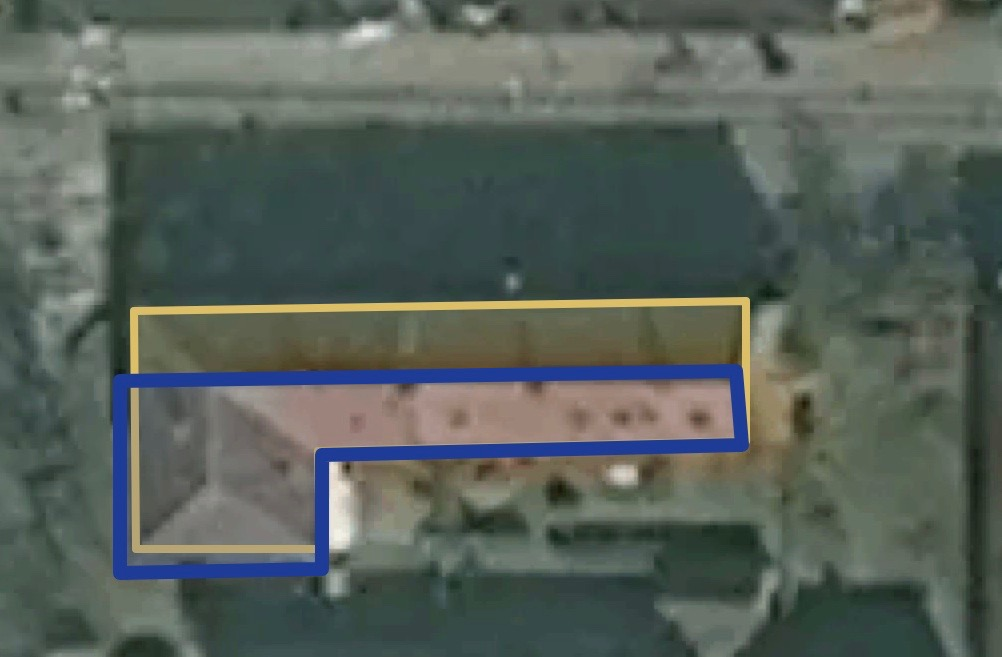
\includegraphics[width=\linewidth]{fig/build3}
		\caption{Both building footprints}
		\label{fig:build3.jpg}
	\end{subfigure}
	\caption{Creating of footprint layers used in question one}
	\label{fig:building_creation_example}
\end{figure}

Position accuracy evaluates how well the coordinate value of a building relates to the reality on the ground. \cite{Fan2014} tested the accuracy of buildings in OSM and concluded with a mean offset of 4.13 m. The low positional accuracy of OSM building footprints data is caused by the limited resolution of Bing map images. By combining shape- and position accuracy in some of the cases used in question one, this study can also determine if participants manage to evaluate both factors. In this study, the participants do not have available information about what the true ground coordinates are. Therefore position accuracy will be examined by shifting one of the layers. The correct positional accuracy will be at the building in the aerial image. 

\section{Web application}
This thesis used an online web-based survey to conduct the experiment. An online survey avoids the cost and effort of printing, distributing, and collecting paper forms. Many people prefer to answer a brief survey displayed on a screen instead of filling in and returning a printed form \citep{Ben2009}. The participants do not have to share the same geographic location as the researcher. 

An online web environment also makes it easier to use interactive maps. An interactive map is necessary to answer question one. It is not possible to have an experiment involving interactive maps on a piece of paper. The web is the obvious way of implementing interactive maps. Making it online, available via URL, makes the distribution faster and easier.

A common web programming language is JavaScript, together with the library React\footnote{React is a open-source JavaScript library for building user interfaces. In React, the displayed data can change without reloading the page. Its main goal is to be fast, simple and scalable.} creates the client side of this thesis application. The client communicates with a server that fetches the task elements from and saves the task results in a PostGIS database. The server is written in Python with the framework Django\footnote{Django is a open-source web framework written in Python. Its primary goal is to ease the creation of complex, database-driven websites.}. The PostGIS database contains the task elements, and also the task results gathered from the participants. 
 
\subsection{React application}
The React application was created to serve the experiment to all participants. It contains all the steps of the experiment. First, the participant registers, giving information about age, gender and answers yes or no on the following two questions: 1) "Do you have experience of working with geospatial data?", 2) "Have you heard of micro-tasking before?". Next, the participant is given an introduction page with a detailed introduction video describing how to answer the two questions, on how to interact with the map and building layers. A training task comes after the instruction video. In the training task the participant solves both questions just like the normal tasks, but it contains different building footprints and two elements to not replicate the other tasks. After the training task, the participant starts with the experiment containing the three tasks, with a short survey after each task. The survey asks the participant to rate the task difficulty between one and five, and if the participant tried his/hers best or was interrupted during the task. The participant can also write a comment. The interfaces for the two questions used in each task is shown in figure \ref{fig:q12} and \ref{fig:q22} in section \ref{sec:experimentquestions}. The registration form and survey interface is shown in figure \ref{fig:client-interface}. 

\begin{figure}[H]
	\centering
	\begin{subfigure}[b]{0.40\textwidth}
		\centering
		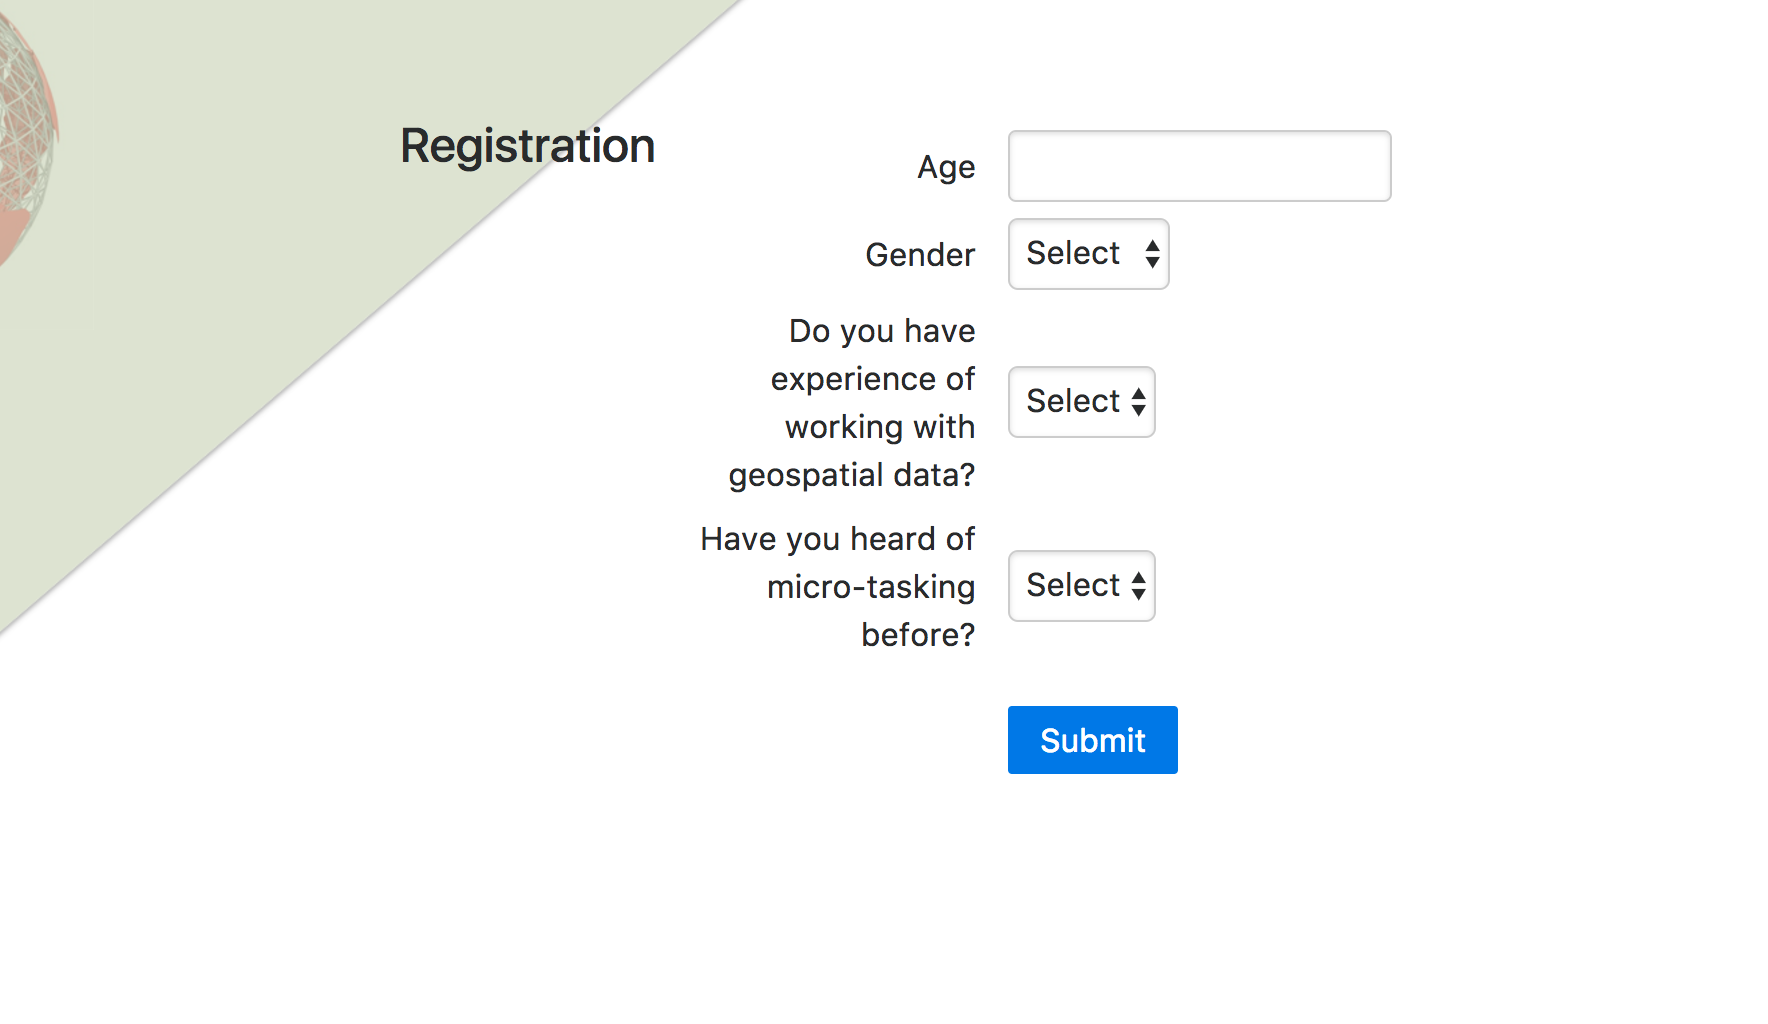
\includegraphics[width=\linewidth]{fig/mt-registration}
		\caption{Registration site}
		\label{fig:mt-registration}
	\end{subfigure}
	\begin{subfigure}[b]{0.35\textwidth}
		\centering
		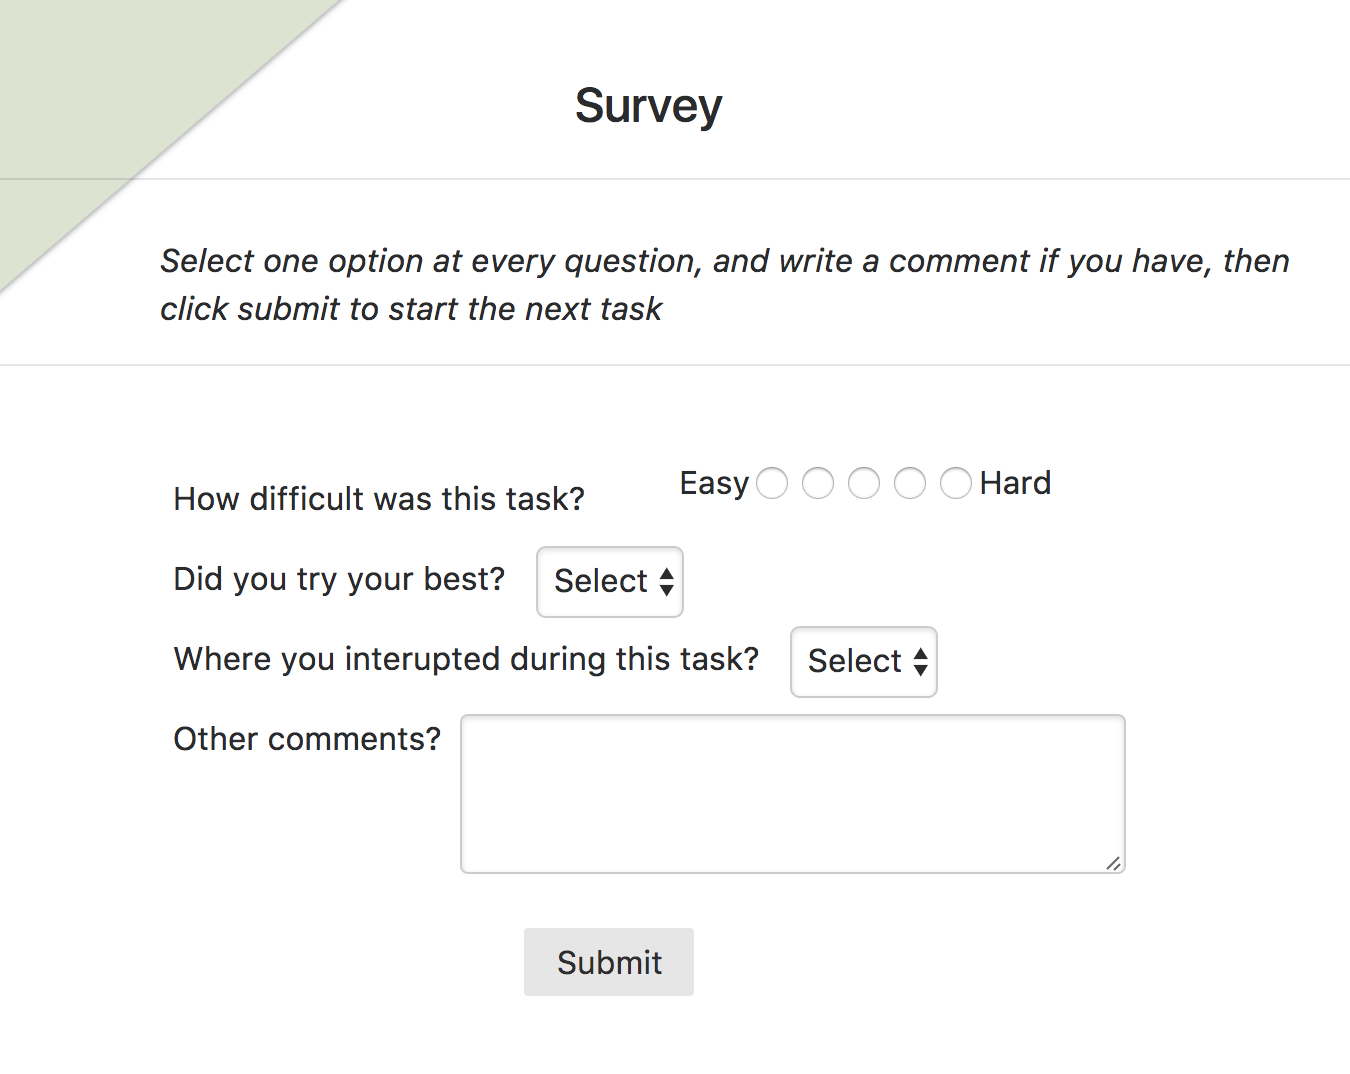
\includegraphics[width=\linewidth]{fig/mt-survey}
		\caption{After each task survey site}
		\label{fig:mt-survey}
	\end{subfigure}
	\caption{Interface for the client application}
	\label{fig:client-interface}
\end{figure}
       
To ensure random and independent observations multiple measurements were implemented during the development of the React application. The main measurements to ensure random, independent observations was:
\begin{itemize}
	\item Random order on the three tasks
	\item Random building footprint pairs in the tasks
	\item Random color on the building footprints
	\item The two building footprints was drawn on the map in a random order
	\item Random order on where the information was positioned in the table
\end{itemize}

When distributing an online experiment, the result can be inconsistent since the researcher is not present to either control the participant or the environment surrounding the participant. The researcher implemented functions securing the completeness of the data. The buttons navigating to the next question and task was disabled until enough building footprints or rows were selected. The participant could not submit their task result before answering both questions correctly. The submit button on the register form and after each task survey only submitted the answers if all fields were answered. If a field was missing, a message appeared, asking the participant to fill out the entire form before submitting. All saved task results were complete in the database thanks to these measurements.

\subsection{Data acquisition}
In this study, the independent variables are: 1) experienced or inexperienced participant, 2) number of elements in the task, 3) age and 4) gender of the participant.  Independent variables are factors we think might influence the results of the study [\citep{Kitchin2000}, p. 49]. When a participant registers at the start of the survey, the independent variables are generated. Participants who answer yes to the question "Do you have experience of working with geospatial data?" are registered as experienced. The independent variables are believed to influence the dependent variables. Dependent variables are factors the study is interested in explaining [\citep{Kitchin2000}, p. 49]. In this study, the dependent variables are: 1) time spent on each question and task, 2) the number of correctly chosen elements in each question and task, and 3) how difficult the participant though the task was. 

The React application generates and saves the task results. In both questions, the time and number of correct elements are registered. The React application has a timer that registers time elapsed on both questions and adds the time measurements together to get the total time spent on the task. The time only reflects how long the participants spent solving the two questions. Time spent loading new layers, moving to the next question, etc., is not included. The building footprints and rows the participant selected is also registered. Before saving the result it counts the number of correctly chosen elements in each question and then adds the number together to get the total number of correctly chosen elements in the task. A participant can maximum have twelve correct elements, six from each question. Total time and number of correct elements are the two primary dependent variables, and they create the basis of the statistical analyses together with the independent variables mentioned above. Participants task results are saved after each task and contain the following information:

\begin{itemize}
	\item Task number (which task)
	\item Task order number (which order)
	\item Time spent on question one 
	\item Time spent on question two
	\item Total time spent on the task
	\item Correct elements in question one
	\item Correct elements in question two
	\item Total correct elements in the task
\end{itemize}
\vspace{0.2cm}

After each task the participants answers a short survey. This information was used to remove task results where the participants was interrupted. The difficulty question can be used to determine if one of the three tasks is preferred by the participants. 

\section{Pilot test}
Testing the experiment before actual use is highly recommended \citep{Ben2009}. A pilot test provides an opportunity to validate the wording of the tasks. It also helps understand the time necessary for completing the survey, which should be communicated to the participants \citep{Schade2015}. The pilot test was carried out on a small sample of users. Results from the pilot test in this thesis was used to make improvements to the actual survey, to the react application and to find errors or weaknesses in the database models.

After the pilot test, the usability was measured. Usability in this thesis was measured with the \textit{System Usability Scale}(SUS) because it gives a subjective measure of usability. The \textit{System Usability Scale} questionnaire consists of ten statements where the participants rate their agreement on a five-point scale \citep{Ben2009}. SUS was developed to be quick and straightforward, but also reliable enough to be able to compare performance changes between versions \citep{Brooke1996}. It is also easy to administer the participants through the usability test, and it can be used on small sample sizes and still give reliable results \citep{Affairs2013}.  

The usability is important to measure. If the participants do not understand how the web application works, they will probably not do the survey since they have to invest time in understanding what to do. %they will either exit the survey or answer the questions in the survey wrong. 
It is also important to get enough participants to do the whole survey and not quit halfway in frustration of not understanding it properly. The \textit{System Usability Scale} can effectively differentiate between usable and unusable systems \citep{Affairs2013}. 

\subsection{Execution of the pilot test}
The pilot test was conducted with a total of eight participants, five experienced and three inexperienced participants aged from 22 to 64 years. The test started with a brief information about this study and the experiment. They were told to "talk out load" during the test and no help or guidance was given to the participants. The participants was observed while they conducted the survey. After the survey a \textit{System Usability Scale} questionnaire was answered by the participants. In the end, the participants were asked to give general feedback on the web application. The SUS score and the feedback were then used to determine the usability of the React application and to determine which improvements to be done.  

\subsection{Results from the pilot test}
The average SUS score was 84.64 out of 100. Anything above 68 is considered above average \citep{Affairs2013}. When adding the SUS score to an adjective rating, a score of 85.5 or higher is described as excellent \citep{Bangor2009}. A score of 84.64 is then described as good/excellent. This result gives a strong indication that the React application is user-friendly. 

All participants thought that the instruction video was confusing. It was short, the instructions went too fast, and it missed voice descriptions. The instructions needed major improvements, which was an important discovery. The purpose of the video is to give the participant an introduction to how to answer the two micro-tasks. It should include important instructions, particularly useful for participants not used to working with interactive maps. 

Overall feedback on question one was that it is hard to understand which building was which because of missing labels, and also to know when a building footprint was selected or not. The lack of labels on the buildings was done on purpose to get the task as realistic as possible to traditional GIS programs (i.e., QGIS). The process of selecting the best fitting building footprint needed improvements. It had to be clearer that one had to click on the layer on the map to choose a footprint, not by using the layer control as some thought. This part was added to the video with voice description, describing in detail how a footprint was selected.

The test data was used to find errors or weaknesses in the database model. The data was extracted from the PostGIS database and saved in CSV files. There were a few errors and weaknesses found during the statistical tests. Changes to the database models were necessary. The task result model was improved by adding four new fields. The additional fields will mainly help with creating plots to interpret the data better and to visualize the different results more easily. 

The average time spent on the survey was 18 minutes. The two oldest participants used on average 33 minutes, while the rest of the participants spent on average 13 minutes to complete the survey. 

In the pilot test, the same building footprints (question one) and information rows (question two) were used in all three tasks. At the end of the pilot test, the author asked the participants if they remembered the buildings and meta information from the previous tasks. $\frac{7}{8}$ answered yes on the question. This information was valuable. If every participant does a better job at the last task, because they remember the elements from earlier tasks, the result will not be as useful. This almost matches the number of participants who remembered the previous elements in the last task. This finding made the author create three different task element groups. Each task will then contain new building footprints and meta information. The three element groups were randomly assigned to each task, to avoid the thee building groups to influence the result. The risk of participants remembering previous task elements disappeared with this decision. 
%Each element group contained six different buildings with two footprints and meta information covering three separate areas. The groups were designed to contain identical element cases. Eighteen footprint pairs and information row pairs were produced because of this decision.

\section[Sample Size]{Determining the sample size}\label{sec:samplesize}
The sample size is influenced by various factors, including the purpose of the study, population size, the risk of selecting a "bad" sample and the allowable sampling error \citep{Israel1992}. 

\begin{figure}[h]
	\centering
	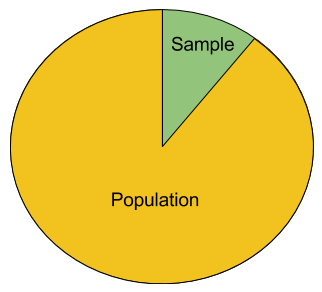
\includegraphics[width=0.35\linewidth]{fig/popsample}
	\caption{Population vs. sample}
	\label{fig:popsample}
\end{figure}

A sample is a collection of observations and is the subset of a population, illustrated in figure \ref{fig:popsample}. The population size in this survey is not easily determined. A population is the collection of individuals of a particular type \citep{Walpole2012}. All individuals with access to a computer and the internet interested in contributing to micro-tasks can be one description of the population. It is important that the sampled population and the target population is similar to one another.

There are three possible ways of determining the sample size in this study. The first option is to use a sample size from a similar study. The risk is to repeat errors that were made in determining the sample for another study. The second option is to rely on published tables, depending on precision, confidence levels, and variability. According to table 1 in the \cite{Israel1992} paper, an accuracy of 0.05, confidence interval of 95\% and a population size greater than 100'000, the necessary sample size is 400. If the accuracy is changed to 0.1, the sample size necessary decreases to 100 \citep{Israel1992}. The numbers found in the table must reflect the number of obtained responses. The last approach is to use formulas to calculate the sample size. The formulas require the standard deviation and how much variance to expect in the response [\citep{Israel1992}, \citep{Smith2013}]. \cite{Israel1992} mentions that table 1 (in his paper) gives a useful guide for determining the sample size and that formulas are used if the study has a different combination of precision and confidence. This study will use the table result since the combinations match this study.

It is important to mention that the quality of the sample is as important as the size. The more variable the sampled data is, the larger the sample size is required \citep{Israel1992}. It is also desirable to choose a random sample, which means that the observations are made independently and random. The main purpose of using a random sample is to obtain correct information about the unknown population parameters \citep{Walpole2012}. 


%Results from the pilot-test can be used to determine the sample size. The sample size tells us how many responses that are needed to make inferences about a population as a whole \citep{Smith2013}. The formula for determining the sample size requires the standard deviation, how much variance to expect in the response \citep{Smith2013}. This standard deviation can be calculated from the pilot test results. Determining sample size is a very important issue because samples that are too large may waste time, resources and money, while samples that are too small may lead to inaccurate result. Equation \ref{eq:samplesize} show how to calculate the sample size, n. 

%\begin{equation}\label{eq:samplesize}
%n = [\frac{z_{\frac{\alpha}{2}}^2 \sigma (1-\sigma)}{e^2}]
%\end{equation}

%Using the results from all participants, excluding the training task, and using data from the column total time, the standardeviation is 184.8 and mean value 156.1 seconds.  
